\documentclass{article}

% For math environments
\usepackage{amsmath, amsfonts}
% For links
\usepackage[hidelinks]{hyperref}
% So space it put between paragraphs
\usepackage{parskip}
% For figures
\usepackage{tikz}
% Set the margins to not be ridiculous
\usepackage[margin=0.75in]{geometry}
% For multiple columns
\usepackage{multicol}
% For controlling enum/itemize spacing and indentation
\usepackage{enumitem}

% For tikz plots
\usepackage{pgfplots}
% This isn't needed but avoids a compiler warning
\pgfplotsset{compat=1.16}

% Allow multi-line equations to be broken across pages
\allowdisplaybreaks

% Use @ as a letter
\makeatletter

% Scale down all tikz coordinates while maintaining font size
\tikzset{every picture/.style={scale=0.45, every picture/.style={}}}


% Macros
% Monospace code
\def\code#1{\texttt{#1}}

% Greek letters
\def\a{\alpha}
\def\b{\beta}
\def\g{\gamma}
\def\d{\delta}
\def\D{\Delta}

% Some common sets
\def\es{\varnothing}
\def\ints{{\mathbb{Z}}}

% Commands that make life easier
\newcommand\gath[1]{\begin{gather} #1 \end{gather}}
\newcommand\gaths[1]{\begin{gather*} #1 \end{gather*}}
\newcommand\ali[1]{\begin{align} #1 \end{align}}
\newcommand\parens[1]{\left( #1 \right)}
\newcommand\squares[1]{\left[ #1 \right]}
\newcommand\braces[1]{\left\{ #1 \right\}}
\newcommand\angles[1]{\left\langle #1 \right\rangle}
\newcommand\deriv[2]{\frac{d #1}{d #2}}
\newcommand\abs[1]{\left| #1 \right|}
\newcommand\floor[1]{\left\lfloor #1 \right\rfloor}
\newcommand\ceil[1]{\left\lceil #1 \right\rceil}
\DeclareMathOperator{\lcm}{lcm}
\def\non{\nonumber \\}
\newcommand\unit[1]{~\mathrm{#1}}
\newcommand\combos[2]{{}_{#1}C_{#2}}

% Set stuff
\def\ss{\subseteq}

% Multiline equation space
\def\mlesp{\hspace{1.2cm}}

% For grid diagrams
\newcommand\gridbox[3]{\draw (#1,#2) rectangle (#1+1,#2+1) node[pos=.5] {#3};}
\newcommand\gridboxh[3]{\draw[fill=red!20] (#1,#2) rectangle (#1+1,#2+1) node[pos=.5] {#3};}
\newcommand\gridboxb[3]{\draw[fill=black] (#1,#2) rectangle (#1+1,#2+1) node[pos=.5] {#3};}
\newcommand\gridsym[3]{\node at (#1+0.5,#2+0.5) {$#3$};}
\newcommand\gridblank[2]{\filldraw[draw=gray, color=gray] (#1,#2) rectangle (#1+1,#2+1);}
\newcommand\gridcirc[2]{\draw (#1 + 0.5,#2 + 0.5) circle (0.25);}
\newcommand\cwlab[3]{
  \def\dd{0.15}
  \draw (#1 + \dd - 0.03, #2 + 1 - \dd) node {\scriptsize #3};
}

\def\bbw{3.5}
\def\bbh{2}
\newcommand\bigbox[3]{\draw (#1*\bbw,#2*\bbh) rectangle (#1*\bbw+\bbw,#2*\bbh+\bbh) node[pos=.5] {#3};}
\newcommand\bbtextr[3]{\node[right] at (#1*\bbw,#2*\bbh+0.5*\bbh) {#3};}
\newcommand\bbtextb[3]{\node[align=center] at (#1*\bbw+0.5*\bbw,#2*\bbh+0.5*\bbh) {#3};}

% Box puzzle stock answer
\newcommand\boxans[1]{
  Logic was used to deduce the solution:

  #1

  This was verified using Python as well as shown to be unique with a brute force approach.
}

% Standard crossnumber grid
\newcommand\crossnumstd[9]{
  \begin{center}
    \begin{tikzpicture}[scale=2]
      \gridbox{0}{2}{#1}
      \gridbox{1}{2}{#2}
      \gridbox{2}{2}{#3}
      \gridbox{0}{1}{#4}
      \gridbox{1}{1}{#5}
      \gridbox{2}{1}{#6}
      \gridbox{0}{0}{#7}
      \gridbox{1}{0}{#8}
      \gridbox{2}{0}{#9}

      % Labels
      \cwlab{0}{2}{1}
      \cwlab{1}{2}{2}
      \cwlab{2}{2}{3}
      \cwlab{0}{1}{4}
      \cwlab{0}{0}{5}
    \end{tikzpicture}
  \end{center}
}

% Multiple numbers
\newcommand\mn[1]{$#1$'s}

% Commands for problems
\newcommand\problem[4]{
\section*{#1}

\textbf{Question:} #3

\textbf{Answer:} #2

\textbf{Explanation:} #4
}
\newcommand\aproblem[4]{\problem{Dec #1}{#2}{#3}{#4}}
\newcommand\cproblem[4]{\problem{Problem #1}{#2}{#3}{#4}}

\newcommand\xref@advent[2]{#1 Advent, Dec~#2 problem}
\newcommand\xref@card[2]{#1 Christmas Card, Problem #2}

% For answered verified with Python
\newcommand{\verified}{This was verified with a brute-force Python program.}

\def\advent@xxi@i{
  The geometric mean of a set of $n$ numbers can be computed by multiplying together all the numbers then computing the $n$th root of the result.

  The factors of $4$ are $1$, $2$ and $4$. The geometric mean of these is 2.

  The factors of $6$ are $1$, $2$, $3$, and $6$. The geometric mean of these is $\sqrt{6}$.

  The geometric mean of all the factors of today's number is $22$.
}

\def\advent@xxi@ii{
  The number $7n$ has $37$ factors (including $1$ and the number itself).
  How many factors does $8n$ have?
}

\def\advent@xxi@iii{
  If you write out the numbers from $1$ to $1000$ (inclusive), how many times will you write the digit $0$?
}

\def\advent@xxi@iv{
  Put the digits $1$ to $9$ (using each digit exactly once) in the boxes so that the sums are correct.
  The sums should be read left to right and top to bottom ignoring the usual order of operations.
  For example, $4 + 3 \times 2$ is $14$, not $10$.
  Today's number is the product of the numbers in the red boxes.

  \grid@advent@xxi@iv{}{}{}{}{}{}{}{}{}
}

\def\advent@xxi@v{
  How many different isosceles triangles are there whose perimeter is $50$ units, and whose area is an integer number of units squared?

  (Two triangles that are rotations, reflections and translations of each other are counted as the same triangle. Triangles with an area of 0 should not be counted.)
}

\def\advent@xxi@vi{
  When $12345$ is divided by today's number, the remainder is $205$.
  When $6789$ is divided by today's number, the remainder is $112$.
}

\newcommand\dec@ai{0.30901699437494745}
\newcommand\dec@aii{0.8090169943749475}
\newcommand\dec@bi{0.5877852522924731}
\newcommand\dec@bii{0.9510565162951535}
\newcommand\decagon[5]{
  \def\ai{\dec@ai*#3+#1}
  \def\aii{\dec@aii*#3+#1}
  \def\bi{\dec@bi*#3+#2}
  \def\bii{\dec@bii*#3+#2}
  \draw (#3+#1, #2) -- (\aii, \bi) -- (\ai, \bii) -- (-\ai, \bii) -- (-\aii, \bi) -- (-#3+#1, #2) -- (-\aii, -\bi) -- (-\ai, -\bii) -- (\ai, -\bii) -- (\aii, -\bi) -- cycle;
  \fill[fill=red] (-\ai, -\bii) -- (#4*#3+#1, #5*#3+#2) -- (\ai, -\bii) -- cycle;
}
\def\advent@xxi@vii{
  The picture below shows eight regular decagons.
  In each decagon, a red triangle has been drawn with vertices at three of the vertices of the decagon.

  \begin{center}
    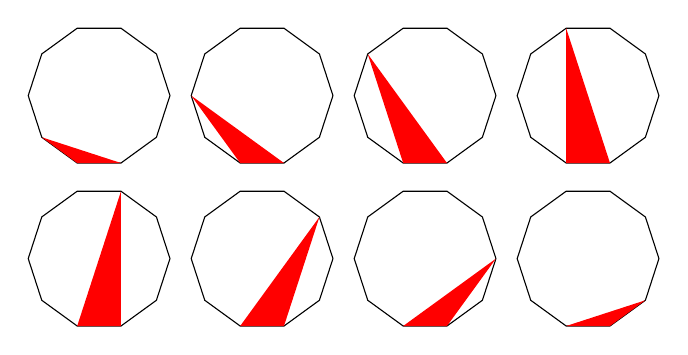
\begin{tikzpicture}
      \def\dr{2}
      \def\spc{2.3*\dr}

      \decagon{0*\spc}{\spc}{\dr}{-\dec@aii}{-\dec@bi}
      \decagon{1*\spc}{\spc}{\dr}{-1}{0}
      \decagon{2*\spc}{\spc}{\dr}{-\dec@aii}{\dec@bi}
      \decagon{3*\spc}{\spc}{\dr}{-\dec@ai}{\dec@bii}

      \decagon{0*\spc}{0}{\dr}{\dec@ai}{\dec@bii}
      \decagon{1*\spc}{0}{\dr}{\dec@aii}{\dec@bi}
      \decagon{2*\spc}{0}{\dr}{1}{0}
      \decagon{3*\spc}{0}{\dr}{\dec@aii}{-\dec@bi}
    \end{tikzpicture}
  \end{center}

  The area of each decagon is $240$.
  What is the total area of all the red triangles?
}

\def\advent@xxi@viii{
  The sum of three integers is $51$.
  The product of the same three integers is $836$. What is the product of largest integer and the second-largest integer?
}

\def\advent@xxi@ix{
  Eve writes down a sequence of consecutive positive integers (she writes more than one number).
  The sum of the numbers Eve has written down is $844$.
  Today's number is the smallest integer that Eve has written down.
}

\def\advent@xxi@x{
  Put the digits $1$ to $9$ (using each digit exactly once) in the boxes so that the sums are correct.
  Today's number is the largest number you can make using the digits in the red boxes.

  \grid@advent@xxi@x{}{}{}{}{}{}{}{}{}
}

\def\advent@xxi@xi{
  The integers are written in a triangle as shown below:
  \begin{center}
    \begin{tabular}{ccccccc}
         &    &    & 1    &    &    &    \\
         &    & 2  & 3    & 4  &    &    \\
         & 5  & 6  & 7    & 8  & 9  &    \\
      10 & 11 & 12 & 13   & 14 & 15 & 16 \\
         &    &    & etc. &    &    &
    \end{tabular}
  \end{center}
  Today's number appears directly above the number $750$ in the triangle of integers.
}

\def\advent@xxi@abgrid{
  \begin{center}
    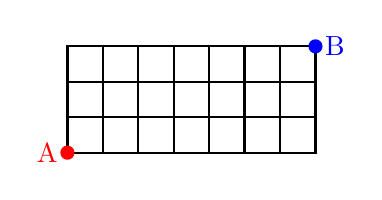
\begin{tikzpicture}
      \def\gs{1}
      % Grid
      \foreach \i in {0,...,6}{
          \foreach \j in {0,...,2}{
              \draw[thick] (\i * \gs, \j * \gs) rectangle (\i * \gs + \gs, \j * \gs + \gs);
            }
        }
      % Points
      \fill[color=red] (0, 0) circle (0.2) node[color=red,left] {A};
      \fill[color=blue] (7*\gs, 3*\gs) circle (0.2) node[color=blue,right] {B};
    \end{tikzpicture}
  \end{center}
}
\def\advent@xxi@xii{
  You start at the point marked A in the picture below. You want to get to the point marked B.
  You may travel \textbf{to the right} or \textbf{upwards} along the black lines.

  \advent@xxi@abgrid

  Today's number is the total number of possible routes to get from A to B.
}

\def\advent@xxi@xiii{
  The diagram below shows three circles and two triangles.
  The three circles all meet at one point.
  The vertices of the smaller red triangle are at the centers of the circles.
  The lines connecting the vertices of the larger blue triangle to the point where all three circles meet are diameters of the three circles.

  \begin{center}
    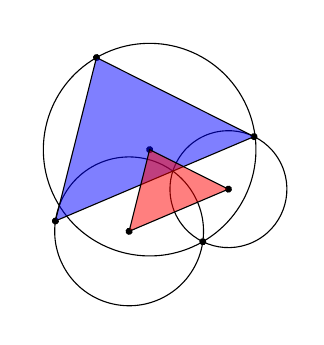
\begin{tikzpicture}[rotate=30,transform shape]
      \def\bcr{3}
      \def\scr{0.55*\bcr}
      \def\sca{34}
      \def\mcr{0.7*\bcr}
      \def\mca{142}
      \def\pr{0.1}

      % Circles
      \draw (0, \bcr) circle (\bcr);
      \draw (\sca: \scr) circle (\scr);
      \draw (\mca: \mcr) circle (\mcr);

      % Points
      \fill (0, 0) circle (\pr);
      \fill (0, \bcr) circle (\pr);
      \fill (0, 2*\bcr) circle (\pr);
      \fill (\sca: \scr) circle (\pr);
      \fill (\sca: 2*\scr) circle (\pr);
      \fill (\mca: \mcr) circle (\pr);
      \fill (\mca: 2*\mcr) circle (\pr);

      % Triangles
      \draw[fill=blue,fill opacity=0.5] (\mca: 2*\mcr) -- (0, 2*\bcr) -- (\sca: 2*\scr) -- cycle;
      \draw[fill=red,fill opacity=0.5] (\mca: \mcr) -- (0, \bcr) -- (\sca: \scr) -- cycle;
    \end{tikzpicture}
  \end{center}

  The area of the smaller red triangle is $226$.
  What is the area of the larger blue triangle?
}

\def\advent@xxi@xiv{
  You start at the point marked A in the picture below.
  You want to get to the point marked B.
  You may travel \textbf{to the right}, \textbf{upwards}, or \textbf{to the left} along the black lines, but you cannot pass along the same line segment more than once.

  \advent@xxi@abgrid

  Today's number is the total number of possible routes to get from A to B.
}

\newcommand\pyramid@advent@xxi@xvi[6]{
  \begin{center}
    \begin{tabular}{cccccc}
      (row 1) &    &    & #1   &    &    \\
      (row 2) &    & #2 &      & #3 &    \\
      (row 3) & #4 &    & #5   &    & #6 \\
              &    &    & etc. &    &
    \end{tabular}
  \end{center}
}
\def\advent@xxi@xv{
  The odd numbers are written in a pyramid.

  \pyramid@advent@xxi@xvi{1}{3}{5}{7}{9}{11}

  What is the mean of the numbers in the 19th row?
}

\newcommand\grid@advent@xxi@xvi[9]{
  \begin{center}
    \begin{tikzpicture}[scale=2]
      \gridbox{0}{2}{#1}
      \gridbox{1}{2}{#2}
      \gridbox{2}{2}{#3}
      \gridbox{0}{1}{#4}
      \gridbox{1}{1}{#5}
      \gridbox{2}{1}{#6}
      \gridbox{0}{0}{#7}
      \gridbox{1}{0}{#8}
      \gridbox{2}{0}{#9}

      % Labels
      \cwlab{0}{2}{1}
      \cwlab{1}{2}{2}
      \cwlab{2}{2}{3}
      \cwlab{0}{1}{4}
      \cwlab{0}{0}{5}
    \end{tikzpicture}
  \end{center}
}
\def\advent@xxi@xvi{
  Each clue in this crossnumber is formed of two parts connected by a logical connective: AND means that both parts are true; NAND means that at most one part is true; OR means that at least one part is true; NOR means that neither part is true; XOR means that exactly one part is true; XNOR means that either both parts are false or both parts are true.
  No number starts with $0$.

  \begin{multicols}{2}
    \grid@advent@xxi@xvi{}{}{}{}{}{}{}{}{}

    \columnbreak

    \begin{enumerate}
      \item \textbf{1A} is a palindrome XNOR \textbf{1D} is a palindrome.
      \item \textbf{1A} is greater than $350$ NOR \textbf{1D} is less than $150$.
      \item \textbf{3D} is odd NAND \textbf{4A} and \textbf{2D} are equal.
      \item \textbf{3D} is prime XOR \textbf{5A} is odd.
      \item \textbf{4A} is a cube AND \textbf{2D} is a cube.
      \item The sum of the digits of \textbf{3D} is $2$ OR the sum of the digits of \textbf{5A} is $5$.
      \item Today's number is \textbf{1D}.
    \end{enumerate}
  \end{multicols}
}

\def\advent@xxi@xvii{
  The digital product of a number is computed by multiplying together all of its digits. For example, the digital product of $6273$ is $252$.

  Today's number is the smallest number whose digital product is $252$.
}

\def\advent@xxi@xviii{
  Put the digits $1$ to $9$ (using each digit exactly once) in the boxes so that the sums are correct.
  The sums should be read left to right and top to bottom ignoring the usual order of operations.
  For example, $4 + 3 \times 2$ is $14$, not $10$.
  Today's number is the product of the numbers in the red boxes.

  \grid@advent@xxi@xviii{}{}{}{}{}{}{}{}{}
}

\def\advent@xxi@xix{
  The equation $352x^3 - 528x^2 + 90 = 0$ has three distinct real-valued solutions.

  Today's number is the number of integers $a$ such that the equation $352x^3 - 528x^2 + a = 0$ has three distinct real-valued solutions.
}

\def\advent@xxi@xx{
  What is the area of the largest area triangle that has one side of length $32$ and one side of length $19$?
}

\newcommand\grid@advent@xxi@xxi[9]{
  \begin{center}
    \begin{tikzpicture}
      \bigbox{0}{3}{#1}
      \bigbox{1}{3}{#2}
      \bigbox{2}{3}{#3}
      \bbtextr{3}{3}{\textbf{today's number}}

      \bigbox{0}{2}{#4}
      \bigbox{1}{2}{#5}
      \bigbox{2}{2}{#6}
      \bbtextr{3}{2}{prime}

      \bigbox{0}{1}{#7}
      \bigbox{1}{1}{#8}
      \bigbox{2}{1}{#9}
      \bbtextr{3}{1}{square}

      \bbtextb{0}{0}{cube}
      \bbtextb{1}{0}{odd}
      \bbtextb{2}{0}{multiple\\of $11$}
    \end{tikzpicture}
  \end{center}
}
\def\advent@xxi@xxi{
  Arrange the digits $1$–$9$ (using each digit exactly once) so that the three digit number in: the middle row is a prime number; the bottom row is a square number; the left column is a cube number; the middle column is an odd number; the right column is a multiple of $11$.
  The $3$-digit number in the first row is today's number.

  \grid@advent@xxi@xxi{}{}{}{}{}{}{}{}{}
}

\def\advent@xxi@xxii{
  There are $12$ ways of placing $2$ tokens on a $2 \times 4$ grid so that no two tokens are next to each other horizontally, vertically or diagonally:

  \begin{center}
    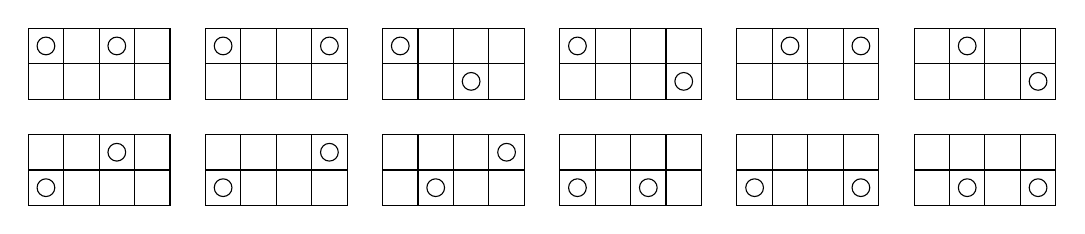
\begin{tikzpicture}
      % Draw all the grids
      \foreach \gi in {0,1}{
          \foreach \gj in {0,...,5}{
              \foreach \i in {0,1}{
                  \foreach \j in {0,...,3}{
                      \gridbox{5*\gj + \j}{3*\gi + \i}{}
                    }
                }
            }
        }

      % Place token circles
      \gridcirc{0}{4}
      \gridcirc{2}{4}
      \gridcirc{5}{4}
      \gridcirc{8}{4}
      \gridcirc{10}{4}
      \gridcirc{12}{3}
      \gridcirc{15}{4}
      \gridcirc{18}{3}
      \gridcirc{21}{4}
      \gridcirc{23}{4}
      \gridcirc{26}{4}
      \gridcirc{28}{3}
      \gridcirc{0}{0}
      \gridcirc{2}{1}
      \gridcirc{5}{0}
      \gridcirc{8}{1}
      \gridcirc{11}{0}
      \gridcirc{13}{1}
      \gridcirc{15}{0}
      \gridcirc{17}{0}
      \gridcirc{20}{0}
      \gridcirc{23}{0}
      \gridcirc{26}{0}
      \gridcirc{28}{0}
    \end{tikzpicture}
  \end{center}

  Today's number is the number of ways of placing $2$ tokens on a $2 \times 21$ grid so that no two tokens are next to each other horizontally, vertically or diagonally.
}

\def\advent@xxi@xxiii{
  I draw the parabola $y = x^2$ and mark points on the parabola at $x = 17$ and $x = -6$.
  I then draw a straight line connecting these two points.

  At which value of $y$ does this line intercept the $y$-axis?
}

\def\advent@xxi@xxiv{
  The digital product of a number is computed by multiplying together all of its digits.
  For example, the digital product of $1522$ is $20$.

  How many $12$-digit numbers are there whose digital product is $20$?
}

\def\card@xxi@i{
  What is the sum of all the odd integers between $0$ and $30$?
}

\def\card@xxi@ii{
  What is the sum of all the odd integers between $0$ and $5668$?
}

\def\card@xxi@iii{
  What is the smallest integer with a digital sum of $28$ and a digital product of $10000$?
}

\def\card@xxi@iv{
  What is the smallest integer with a digital sum of $41$ and a digital product of $432000$?
}

\def\card@xxi@v{
  What is the area of the largest area dodecagon that will fit inside a circle with area $111185 \pi$?
}

\def\card@xxi@vi{
  What is the area of the largest area heptagon that will fit inside a semicircle with area $115185 \pi$?
}

\def\card@xxi@vii{
  How many terms are there in the (simplified) expansion of $(x + y + z)^2$?
}

\def\card@xxi@viii{
  How many terms are there in the (simplified) expansion of $(x + y + z)^{41172}$?
}

\def\card@xxi@ix{
  What is the largest integer that cannot be written as $4a + 5b$ for non-negative integers $a$ and $b$?
}

\def\card@xxi@x{
  What is the largest integer that cannot be written as $83409a + 66608b$ for non-negative integers $a$ and $b$?
}

\def\card@xxi@xi{
  How many positive integers are there below $100$ whose digits are all non-zero and different?
}

\def\card@xxi@xii{
  How many positive integers are there whose digits are all non-zero and different?
}

\def\card@xxi@xiii{
  What is the only integer for which taking the geometric mean of all its factors (including $1$ and the number itself) gives $2$?
}

\def\card@xxi@xiv{
  What is the only integer for which taking the geometric mean of all its factors (including $1$ and the number itself) gives $25$?
}

\input{boxes}

\begin{document}

\title{Matthew Scroggs Advent Calendar 2024 Answers}
\author{Dan Whitman}
\date{}

\maketitle

Sync answers: \href{http://mscroggs.co.uk/adventcode/O7IMqY4B}{http://mscroggs.co.uk/adventcode/O7IMqY4B}

\aproblem{1}{144}{\advent@xxiv@i}{
  Let $A$ denote any set of five distinct positive integers that sums to $16$.
  If $1 \notin A$ then the smallest possible sum would be
  \gath{
    2 + 3 + 4 + 5 + 6 = 20.
  }
  As this exceeds $16$, it must be that $1 \in A$.
  Similarly, if $2 \notin A$, then the smallest possible sum is
  \gath{
    1 + 3 + 4 + 5 + 6 = 19,
  }
  which again exceeds $16$, so that it must be that $2 \in A$ as well.
  What if $3 \notin A$?
  Then, again, the smallest sum becomes
  \gath{
    1 + 2 + 4 + 5 + 6 = 18,
  }
  and hence $3 \in A$ as well.
  Lastly, if $4 \notin A$, then the smallest sum becomes
  \gath{
    1 + 2 + 3 + 5 + 6 = 17
  }
  so that $4$ must be in $A$.

  Therefore, $A = \braces{1, 2, 3, 4, n}$ where $n$ is some unknown positive integer.
  Clearly we have
  \gath{
    1 + 2 + 3 + 4 + n = 16 \non
    10 + n = 16 \non
    n = 6
  }
  so that it has to be that
  \gath{
    A = \braces{1, 2, 3, 4, 6}.
  }
  The product of these is then of course $1 \cdot 2 \cdot 3 \cdot 4 \cdot 6 = 144$, which is our answer.
  This was also validated using a brute force Python program.
}

\aproblem{2}{202}{\advent@xxiv@ii}{
  For a pair of $N$-sided dice, let $f(N)$ denote the smallest even number that \emph{cannot} be obtained by the product of a roll of the dice.
  The general claim is that $f(N)$ is $2a$ where $a$ is the smallest prime number greater than $N$, though we will not prove this in full generality.

  So, for the $N = 6$ example, the smallest prime larger than $6$ is of course $a = 7$ so that $f(6) = 2a = 2 \cdot 7 = 14$.
  For $N = 100$, the smallest prime larger than $100$ is clearly $a = 101$ so that our answer becomes $f(100) = 2a = 2 \cdot 101 = 202$.

  We \emph{will} prove this special case when $a = N + 1$, which applies to both the example and our actual problem.
  First, let $n = 2a$, noting that $n$ has only the nontrivial factors $2$ and $a$ since $a$ is prime.
  A roll of the $N$-sided pair of dice cannot produce this even number as a product because the pair would have to be either a $1$ and an $n$ or a $2$ and an $a$.
  However, we have that
  \gath{
    N < N + 1 = a < 2a = n
  }
  so that the neither of the required larger factors of $n$ or $a$ appear on any side of either die.

  Now, suppose that $m = 2b$ is an even number less than $n$.
  Then of course
  \gath{
    2b = m < n = 2a \non
    b < a \non
    b < N + 1
  }
  so that $b \leq N$ and so is a number on the side of each die.
  Hence, the product of the roll of a $2$ and a $b$ is of course $2b = m$ so that this is attainable as the product of a roll.
  Since $m < n$ was arbitrary, this shows that $f(N) = n$ is the \emph{smallest} even number that cannot be obtained from the pair of dice.

  These results were verified with a brute force Python program.
}

\aproblem{3}{377}{\advent@xxiv@iii}{
  This is similar to the 2018, Dec~1 problem and the general approach will be the same.
  For any positive integer $n$, let $f(n)$ denote the number of ways to write $n$ as a sum of positive odd integers.
  For reasons that will become clear momentarily, we set $f(0) = 1$.
  Clearly also $1 = 1$ and $2 = 1 + 1$ are the only valid ways to write those numbers so that $f(1) = f(2) = 1$.

  Now, if $n = 2m+1$ is odd, then the first number in the sum can be one of $m+1$ odd numbers, including $n$ itself.
  Specifically, these are $2k+1$ where $0 \leq k \leq m$.
  Once this number is chosen via $k$, the remaining value of the sum is
  \gath{
    n - (2k+1) = (2m + 1) - (2k + 1) = 2(m-k)
  }
  such that all the numbers still sum to $n$, and there are of course $f\squares{2(m-k)}$ ways to express this value as the sum of odd numbers.
  Thus, the total number of ways to express $n$ is to sum over all the choices of $k$, which becomes the recursive formula
  \gath{
    f(2m+1) = \sum_{l=0}^m f\squares{2(m-l)}. \label{eqn:03:odd:pre}
  }
  We can simplify this by setting $k = m-l$ so that $l = 0 \to k = m$ and $l = m \to k = 0$, and hence
  \gath{
    f(2m+1) = \sum_{k=0}^m f(2k). \label{eqn:03:odd}
  }
  Note that the first number in the sum being $n$ itself corresponds to $l = m$ in \eqref{eqn:03:odd:pre} and $k = 0$ in \eqref{eqn:03:odd} so that the remaining value is $0$ and hence $f(2k) = f(0) = 1$ since overall there is only one of these sums.
  Thus, we set $f(0) = 1$ above to make \eqref{eqn:03:odd:pre} and \eqref{eqn:03:odd} more concise.

  Now suppose that $n = 2m$ is even.
  Here there are $m$ choices for the first number, namely the odd numbers $2k+1$ where $0 \leq k \leq m-1$.
  The remaining sum value is then
  \gath{
    n - (2k+1) = 2m - 2k - 1 = 2(m-k) - 1.
  }
  Following the same line of reasoning as the odd case, the recursive formula becomes
  \gath{
    f(2m) = \sum_{l=0}^{m-1} f\squares{2(m-l)-1}.
  }
  We can again change variables to $k = m-l$ so that $l = 0 \to k = m$ and $l = m-1 \to k = 1$, and hence
  \gath{
    f(2m) = \sum_{k=1}^m f(2k-1). \label{eqn:03:even}
  }

  Now, if again $n = 2m+1$ is odd then we clearly have
  \ali{
    n - 1 &= 2m \label{eqn:03:onmo} \\
    n - 2 &= 2m - 1 = 2m - 1 + 2 - 2 = 2(m-1) + 1.
  }
  Therefore, by \eqref{eqn:03:odd}, we get
  \gath{
    f(n-2) = f\squares{2(m-1)+1} = \sum_{k=1}^{m-1} f(2k) \label{eqn:03:omt}
  }
  so that
  \ali{
    f(n) &= f(2m+1) = \sum_{k=0}^m f(2k) \non
    &= \sum_{k=0}^{m-1} f(2k) + f(2m) \non
    &= f(n-2) + f(n-1)
  }
  by \eqref{eqn:03:omt} and \eqref{eqn:03:onmo}, which is the recursive Fibonacci relation!
  What happens though when $n = 2m$ is even?
  In this case we have
  \ali{
    n - 1 &= 2m - 1 \label{eqn:03:emo} \\
    n - 2 &= 2m - 2 = 2(m-1)
  }
  and
  \gath{
    f(n-2) = f\squares{2(m-1)} = \sum_{k=1}^{m-1} f(2k-1) \label{eqn:03:emt}
  }
  by \eqref{eqn:03:even}.
  Hence,
  \ali{
    f(n) &= f(2m) = \sum_{k=1}^m f(2k-1) \non
    &= \sum_{k=1}^{m-1} f(2k-1) + f(2m-1) \non
    &= f(n-2) + f(n-1)
  }
  by \eqref{eqn:03:emt} and \eqref{eqn:03:emo}, which is the same relation!

  Therefore, we have the standard Fibonacci sequence:
  \ali{
    f(1) &= 1 \non
    f(2) &= 1 \non
    f(n) &= f(n-1) + f(n-2).
  }
  Noting that we can calculate the example at $f(5) = 5$, it is then largely trivial to continue the sequence to calculate our answer of $f(14) = 377$.

  These results were verified with a brute force Python program.
}

\aproblem{4}{169}{\advent@xxiv@iv}{
  We know from the 2021, Dec~1 problem that \emph{only} such number is $13^2 = 169$.
  This was verified using a brute force Python program.
}

\aproblem{5}{179}{\advent@xxiv@v}{
  We can leverage the results of the 2021, Dec~9 problem.
  There, the sum of the $n$ consecutive integers starting at (and including) $a$ was derived to be
  \gath{
    \sum_{k=a}^{a+n-1} k = \frac{1}{2} n (n + 2a - 1) \label{eqn:05:sum}
  }
  Suppose that this sum is given as $s$ and that $n$ is also known.
  Then we can solve \eqref{eqn:05:sum} for $a$ to get
  \gath{
    \frac{1}{2} n (n + 2a - 1) = s \non
    n + 2a - 1 = \frac{2s}{n} \non
    2a = \frac{2s}{n} - n + 1 \non
    a = \frac{s}{n} + \frac{1 - n}{2} \label{eqn:05:solved}
  }
  In our case we have $n = 11$ and $s = 2024$ so that \eqref{eqn:05:solved} evaluates to our answer $a = 179$.
}

\aproblem{6}{990}{\advent@xxiv@vi}{
  Suppose that $a_k$ is the $k$-digit number whose digits are all $9$, which is to say that $a_k = 10^k - 1$.
  Also, let $e(m)$ denote the number of digital nines in $m$.
  We show these below for $1 \leq k \leq 10$:

  \begin{center}
    \begin{tabular}{c|c|c|c}
      $k$ & $a_k$      & $a_k^3$                        & $e(a_k^3)$ \\
      \hline
      1   & 9          & 729                            & 1          \\
      2   & 99         & 970299                         & 3          \\
      3   & 999        & 997002999                      & 5          \\
      4   & 9999       & 999700029999                   & 7          \\
      5   & 99999      & 999970000299999                & 9          \\
      6   & 999999     & 999997000002999999             & 11         \\
      7   & 9999999    & 999999700000029999999          & 13         \\
      8   & 99999999   & 999999970000000299999999       & 15         \\
      9   & 999999999  & 999999997000000002999999999    & 17         \\
      10  & 9999999999 & 999999999700000000029999999999 & 19         \\
    \end{tabular}
  \end{center}

  In the context of the digital sum of $a_k^3$, we can observe that $a_k^3$ has one seven, one two, some irrelevant number of zeros, and some number of nines.
  Though we do not attempt to prove it, it seems that the number of nines $e(a_k^3)$ is simply the odd numbers.
  That is
  \gath{
    e(a_k^3) = 2k - 1.
  }
  Letting $s(m)$ denote the digital sum of $m$, the digital sum of $a_k^3$ should then be
  \ali{
    s(a_k^3) &= 9e(a_k^3) + 7 + 2 = 9e(a_k^3) + 9 \non
    &= 9(2k - 1) + 9 = 9(2k - 1 + 1) \non
    &=18k
  }
  This result was verified using a Python program for all $1 \leq k \leq 1000$.
  This of course included our particular case of $s(n) = s(a_{55}^3) = 18 \cdot 55 = 990$, which is our answer.
}

\aproblem{7}{119}{\advent@xxiv@vii}{
  In what follows, we take 12 o'clock to be at zero degrees, with increasing angles going clockwise, in opposition to the standard counter-clockwise on the polar plane.

  Regarding the minute hand, each revolution of the hand around the clock face is an hour, which is of course 60 minutes.
  Thus, each minute advances the minute hand by $m = 360/60 = 6\unit{degrees}$.
  This means that position of the minute hand at 08:22 would be $p_m = 22m = 132$ degrees relative to (12 o'clock).

  For the hour hand, each revolution around the clock face is $12$ hours, during which time $60 \cdot 12 = 720$ minutes pass.
  Hence, every minute advances the hour hand by $h = 360 / 720 = 1/2$ a degree.
  The time 08:22 is of course 8 hours and 22 minutes past midnight (12 o'clock on the clock face), which is equivalent to $m_h = 60 \cdot 8 + 22 = 502$ total minutes.
  Thus, the position of the hour hand is $p_h = m_h h = 502 /2 = 251$ degrees.

  The angle between them is then $\abs{p_h - p_m} = \abs{251 - 132} = 119$ degrees, which is indeed obtuse.
}

\aproblem{8}{575}{\advent@xxiv@viii}{
  Suppose that we have $n$ points in a plane forming $T(n)$ triangles with a convex overall boundary.
  If we then add a point somewhere \emph{inside} one of the triangles (i.e. not on an edge or at a vertex) and connect this new point to each of the three vertices of the triangle, then this divides that triangle into three smaller triangles.
  Hence, we have created two additional triangles (the third simply replacing the one that was subdivided) so that
  \gath{
    T(n+1) = T(n) + 2. \label{eqn:05iii:rec}
  }
  It is easy to see that this is a way to create the \emph{most} new triangles since putting the new point \emph{outside} the entire shape will only create one new triangle since the shape is convex.
  The point could also be added on the edge of an existing triangle (but not on an existing vertex) as this subdivides \emph{two} original triangles each into two sub-triangles, again adding two additional triangles overall.

  Now, for three points, clearly the maximum number of triangles is simply one, noting that this is also always convex.
  Therefore, we have
  \gath{
    T(3) = 1. \label{eqn:05iii:base}
  }

  From \eqref{eqn:05iii:rec} and \eqref{eqn:05iii:base} it is easy to deduce that
  \gath{
    T(n) = 2n - 5. \label{eqn:05iii:closed}
  }
  This is also easy to prove using induction.
  First, clearly for $n = 3$ we have
  \gath{
    T(n) = T(3) = 2 \cdot 3 - 5 = 6 - 5 = 1,
  }
  which comports with \eqref{eqn:05iii:base}.
  Now suppose that \eqref{eqn:05iii:closed} is true for $n$.
  Then we have
  \ali{
    T(n+1) &= T(n) + 2 & \text{(by \eqref{eqn:05iii:rec})} \non
    &= 2n - 5 + 2 & \text{(by the induction hypothesis)} \non
    &= 2(n+1) - 5,
  }
  which shows that \eqref{eqn:05iii:closed} is true for $n+1$ as well, completing the induction.

  Finally, the answer we seek is then $T(290) = 2 \cdot 290 - 5 = 575$, noting that also $T(4) = 2 \cdot 4 - 5 = 3$ as expected per the example and diagram above.
}

\aproblem{9}{252}{\advent@xxiv@ix}{
  \boxans{\gridsol@advent@xxiv@ix}
}

\aproblem{10}{495}{\advent@xxiv@x}{
  We can ignore $100$ since this is clearly not a palindrome.
  Thus, we consider all two-digit numbers: $10$ through $99$.
  It is apparent that these can be a palindrome if and only if both digits are the same.
  These are exactly the numbers $x_n = 10n + n$ where $1 \leq n \leq 9$.
  Hence, the sum of these is
  \gath{
    \sum_{n=1}^9 x_n = \sum_{n=1}^9 (10n + n) = \sum_{n=1}^9 11n = 11 \sum_{n=1}^9 n = 11 \frac{9 \cdot 10}{2} = 55 \cdot 9 = 495,
  }
  which is our answer.

  This result was verified with a brute force Python program.
}

\aproblem{11}{210}{\advent@xxiv@xi}{
  Suppose that we consider the integers between $1$ and an odd $N = 2k+1$ inclusive.
  Consider the number of sets of odd size $n = 2l+1$ whose median value is $m$ (where of course $1 \leq m \leq N$).
  Since $m$ is the median value, there must be $l$ values less than $m$ and $l$ values greater than $m$.
  For values less than $m$ there are $m-1$ possible numbers, from which we must choose $l$.
  Thus, there are
  \gath{
    P_<(m, l) = \binom{m-1}{l}
  }
  possibilities.
  For values greater than $m$ there are $N - m$ possible numbers, from which $l$ must be chosen again.
  Here there are
  \gath{
    P_>(m, l) = \binom{N-m}{l} = \binom{2k+1-m}{l}
  }
  possibilities.
  Since these choices are independent of each other, there are clearly
  \gath{
    P(m, l) = P_<(m, l) \cdot P_>(m, l) = \binom{m-1}{l} \binom{2k+1-m}{l}
  }
  total possible sets of $2l +1$ elements such that $m$ is the median.
  It then follows that the total number of possible sets of integers in $[1, 2k+1]$ where $m$ is the median is
  \gath{
    S(k, m) = \sum_{l=0}^k P(m, l) = \sum_{l=0}^k \binom{m-1}{l} \binom{2k+1-m}{l}.
  }
  For the example, this evaluates to the expected $S(2, 3) = 6$, noting that here $N = 5 = 2 \cdot 2 + 1$.
  For the main problem, we have $N = 11 = 2 \cdot 5 + 1$ so that $S(5, 5) = 210$ is our answer.
  These were calculated using Python.
}

\aproblem{12}{281}{\advent@xxiv@xii}{
  Suppose that the original three-digit number has digits $d_2 d_1 d_0$, which is to say that the number itself is $100d_2 + 10d_1 + d_0$.
  First, it must be that the digit that is removed is the least significant $d_0$ since otherwise the sum of the numbers would end in an even digit.
  Hence, we have the following addition
  \begin{center}
    \begin{tabular}{c@{}c@{}c@{}c}
        & $d_2$ & $d_1$ & $d_0$ \\
      + &       & $d_2$ & $d_1$ \\
      \hline
        & 3     & 0     & 9
    \end{tabular}
  \end{center}
  Since $9 + 9 = 18 < 19$, the ones place column can only sum to $9$ and not $19$, thus there cannot be a carry to the tens place.
  Moreover, noting that $d_2$ cannot be zero (since then we would not have a three-digit number at all), the tens place column can sum to zero only if the digits $d_1$ and $d_2$ sum to $10$ since there is no carried value to account for.

  It then follows that there is a carried value of $1$ added to $d_2$ in the hundreds place so that $d_2 + 1 = 3$ and, therefore, $d_2 = 2$.
  From before, we then have $d_1 + d_2 = d_1 + 2 = 10$ so that $d_1 = 8$.
  Lastly, we know that $d_0 + d_1 = d_0 + 8 = 9$, thus $d_0 = 1$.
  So our addition has to be
  \begin{center}
    \begin{tabular}{c@{}c@{}c@{}c}
        & 2 & 8 & 1 \\
      + &   & 2 & 8 \\
      \hline
        & 3 & 0 & 9
    \end{tabular}
  \end{center}
  and Holly's original three-digit number is of course $281$.
}

\aproblem{13}{997}{\advent@xxiv@xiii}{
  \boxans{\crossnumstd{9}{9}{7}{4}{7}{0}{2}{3}{5}}
}

\aproblem{14}{625}{\advent@xxiv@xiv}{
  Let $D(n)$ denote $15^n$ modulo $1000$ for a natural number $n$, so that it is effectively only the last three digits of $15^n$.
  We will prove that
  \gath{
    D(n) =
    \begin{cases}
      375 & \text{$n$ is odd}  \\
      625 & \text{$n$ is even}
    \end{cases} \label{eqn:14:dn}
  }
  for all $n \geq 3$.
  We show this by induction on $n$.
  First, clearly
  \gath{
    D(3) = 15^3 \pmod{1000} = 3375 \pmod{1000} = 375
  }
  so that \eqref{eqn:14:dn} holds in the base case.
  Now assume that \eqref{eqn:14:dn} holds for $n$.
  If $n$ is odd then $D(n) = 15^n \pmod{1000} = 375$ so that
  \ali{
    D(n+1) &= 15^{n+1} \pmod{1000} \non
    &= 15 \cdot 15^n \pmod{1000} \non
    &= 15 \cdot 375 \pmod{1000} \non
    &= 5625 \pmod{1000} \non
    &= 625,
  }
  noting that $n+1$ is even since $n$ is odd.
  On the other hand, if $n$ is even, then $D(n) = 15^n \pmod{1000} = 625$, and hence
  \ali{
    D(n+1) &= 15^{n+1} \pmod{1000} \non
    &= 15 \cdot 15^n \pmod{1000} \non
    &= 15 \cdot 625 \pmod{1000} \non
    &= 9375 \pmod{1000} \non
    &= 375,
  }
  noting that $n+1$ is odd since $n$ is even.
  Thus $D(n+1)$ holds for either parity of $n$, completing the induction.

  Our answer is then
  \gath{
    15^{1234567890} \pmod{1000} = D(1234567890) = 625
  }
  since $1234567890$ is even.
}

\aproblem{15}{976}{\advent@xxiv@xv}{
  Let $R(n)$ denote the number obtained by reversing the digits of $n$.
  We can simply enumerate the first ten square numbers and the product of the square and its reversed-digit number:
  \begin{center}
    \begin{tabular}{c|cc|cc}
      $n$ & $n^2$ & $R(n^2)$ & $n^2 \cdot R(n^2)$ & Three digits? \\
      \hline
      1   & 1     & 1        & 1                  & No            \\
      2   & 4     & 4        & 16                 & No            \\
      3   & 9     & 9        & 81                 & No            \\
      4   & 16    & 61       & 976                & Yes           \\
      5   & 25    & 52       & 1300               & No            \\
      6   & 36    & 63       & 2268               & No            \\
      7   & 49    & 94       & 4606               & No            \\
      8   & 64    & 46       & 2944               & No            \\
      9   & 81    & 18       & 1458               & No            \\
    \end{tabular}
  \end{center}
  The next square is $10^2 = 100$ which cannot be used (since it ends in not one, but two zeros), then comes $11^2 = 121$, which is palindromic so that $121 \cdot 121 = 14641$ is itself a square number.
  Regardless of these interesting properties, clearly we are getting into products that are far too large, and so there is no need to continue.
  Looking at the table above, evidently there is only \emph{one} square number such that the product of it and its reversed-digit number is exactly three digits!
  Thus, our answer must be $4^2 \cdot R(4^2) = 16 \cdot 61 = 976$.
}

\aproblem{16}{336}{\advent@xxiv@xvi}{
  \boxans{\gridsol@advent@xxiv@xvi}
}

\aproblem{17}{972}{\advent@xxiv@xvii}{
Let $N(n)$ denote the number of factors of a positive integer $n$.
If $n$ has the prime factorization of
\gath{
n = \prod_{i=1}^N p_i^{e_i},
}
then the number of factors is
\gath{
  N(n) = \prod_{i=1}^N (e_i + 1).
}
So, for the example, the prime factorization of $40$ is $2^3 \cdot 5$ so that
\gath{
  N(40) = (3+1)(1+1) = 4 \cdot 2 = 8.
}
Our actual number is already given in terms of its prime factorization, i.e.
\gath{
  n = 2^{26} \cdot 5 \cdot 7^5 \cdot 11^2,
}
so that clearly
\gath{
  N(n) = (26+1)(1+1)(5+1)(2+1) = 27 \cdot 2 \cdot 6 \cdot 3 = 972
}
is our answer.
}

\aproblem{18}{756}{\advent@xxiv@xviii}{
  Let $\a = 28$, so that we have
  \gath{
    \frac{\a k}{\a + k} = m \label{eqn:18:m}
  }
  for some integer $m$, noting that $m$ must be positive since $k$ is (since then both $\a k > 0$ and $\a + k > 0$).
  We can rearrange \eqref{eqn:18:m} to obtain
  \gath{
    k = \frac{\a m}{\a - m}. \label{eqn:18:k}
  }
  Now, the denominator must be positive since we would like our $k$ to be positive (and finite!).
  Hence, it has to be that $0 < a - m$ so that $m < \a$.
  Moreover, larger $m$ will result in a larger numerator (i.e. $\a m$) and a smaller denominator (i.e. $\a - m$) so that the fraction $k$ will be larger.
  That is, we want $m$ to be as large as it can be since we are interested in the largest qualifying $k$.

  Since also $m < \a$, how about the largest possible $m$ of $m = \a - 1 = 27$?
  Indeed, $m = 27$ results in $k = 756$ from \eqref{eqn:18:k}, noting that this simply makes the denominator $1$ so that of course $k = \a m = \a (\a - 1)$ is an integer.
  Hence, $k = 756$ has to be the answer we seek.
}

\aproblem{19}{TODO}{\advent@xxiv@xix}{
  TODO
}

\end{document}
